% !TeX program = pdflatex
% ============================================================================
%  Landing Self-Evidencing: What Actually Ran on a Domestic-Process Mobile NPU
%  IEEEtran conference draft — 2026-09-21
%
%  数字来源：lpr-kirin8020/docs/evidence-index.md（唯一来源）
%  守卫：    lpr-kirin8020-app/tools/verify_published_numbers.py（不过则不许发布）
%  图：      paper/figures/（由 lpr-kirin8020-app/tools/make_figures.py 生成）
%
%  禁止出现：任何 NPU 利用率数字（ADR-0003）。
% ============================================================================
\documentclass[conference]{IEEEtran}
\IEEEoverridecommandlockouts

\usepackage{cite}
\usepackage{amsmath,amssymb,amsfonts}
\usepackage{graphicx}
\usepackage{textcomp}
\usepackage{xcolor}
\usepackage{booktabs}
\usepackage{url}
\usepackage[hidelinks]{hyperref}

\graphicspath{{../figures/}}

\newcommand{\landed}{\texttt{LANDED}}
\newcommand{\reqf}{\texttt{req}}
\newcommand{\fbf}{\texttt{fallback}}

\begin{document}

\title{Landing Self-Evidencing:\\
Establishing What Actually Ran on a Domestic-Process Mobile NPU}

\author{
\IEEEauthorblockN{Shusen Yang}
\IEEEauthorblockA{\textit{Independent Researcher}\\
China\\
\texttt{2667199938@qq.com}}
}

\maketitle

\begin{abstract}
Mobile NPUs are now ubiquitous, but on some vendor platforms the most basic
question about a deployment---\emph{did the work actually run on the NPU}---cannot
be answered by measurement. On the platform studied here, NPU utilisation is not
exposed to applications, not exposed to the on-device debug shell, and not
exposed by any vendor profiling template. Worse, backend placement is silent:
a model requested on the NPU may fall back to the CPU with no error code, and a
model that does land on the NPU may compute a different answer than its CPU
counterpart. We present \emph{landing self-evidencing}, a measurement protocol
that makes backend placement readable from raw logs rather than asserted from
configuration, and apply it to a four-stage Chinese licence-plate recognition
pipeline on a Kirin 8020 (HarmonyOS 6, MindSpore Lite~$\rightarrow$~NNRT). Three
findings follow. (i)~The protocol is effective: it detected a pure
pre-processing defect that was invisible at the output layer, and it correctly
attributed that defect to the input rather than to the accelerator.
(ii)~NPU operator supportability is a \emph{model $\times$ toolchain} joint
property, not a hardware property: the same 51 operator probes that the NNRT
path partly rejects pass 51/51 through the CANN toolchain, including
\texttt{ConvTranspose}, which cannot even be converted on the NNRT side.
(iii)~For this pipeline, switching the recogniser's backend changed 0\% of
outputs and the detector's 0.1\% over 1{,}000 real vehicle images---yet a paired
McNemar test shows the backend \emph{is} an accuracy variable
($+3.2$\,pp, $p<0.0001$), while plate length costs an order of magnitude more
($-6.6$\,pp). We report these results together with their boundaries, including
one where a sustained-load experiment failed to reach the thermal regime it was
designed to probe.
\end{abstract}

\begin{IEEEkeywords}
on-device inference, heterogeneous inference, mobile NPU, HarmonyOS, MindSpore
Lite, NNRT, operator delegation, licence plate recognition, measurement
methodology
\end{IEEEkeywords}

% ============================================================================
\section{Introduction}

Deploying a neural network on a mobile NPU is normally presented as a
performance question: how much faster is the accelerator than the CPU? On the
platform we study, that framing breaks down before it can be applied.

Three properties of the platform obstruct it. First, \textbf{placement is
silent}. A session created with an NPU target may be served by the CPU, and
nothing in the application-visible result records which happened; a
configuration file describing the intended backend is not evidence about the
executed backend. Second, \textbf{acceleration is not guaranteed by placement}.
Across a prior characterisation of the same device family, measured speed-ups
ranged from $13.11\times$ down to $0.98\times$, with small models losing to the
CPU because a fixed per-delegation cost cannot be amortised. Third, and most
awkward, \textbf{a model can land on the NPU and compute the wrong answer
without an error code}. During an early run, a detector served by the NPU read
a plate as \texttt{Su\,E05172} where the CPU read \texttt{Su\,ED5172}; both runs
returned success.

Under these conditions the ordinary verification instrument is unavailable. On
this platform NPU utilisation is not exposed to applications, is not available
through the device debug shell, and has no vendor profiling template; the only
NPU-related counter available is a \emph{temperature}, not a load. We therefore
treat this as a measurement problem rather than a tuning problem, and ask:
\emph{what can be honestly established about which hardware executed a given
inference, and what follows for the engineering decisions that depend on it?}

\subsection{Contributions}

\begin{itemize}
\item \textbf{C1 --- Landing self-evidencing.} A protocol that makes backend
placement readable from raw logs: every inference records the requested backend
(\reqf), the observed backend (\landed), and any fallback transition (\fbf), and
these are read together with a tensor fingerprint and a CPU differential. We
describe the protocol, show that it caught a real defect, and---equally
important---show the case where it was initially \emph{misread}, and how that
misreading was corrected (\S\ref{sec:protocol}).

\item \textbf{C2 --- Operator coverage is a model $\times$ toolchain joint
property.} We contrast two toolchains targeting the same silicon. On the NNRT
path, 16 of 36 operator probes are rejected when compiled standalone. On the
CANN path, the same family of probes passes 51/51. We further characterise the
mechanism---operators rejected in isolation are still carried onto the NPU as
fusion neighbours of an adjacent convolution---and are explicit that this
mechanism is currently supported by correlation, not by a controlled causal
experiment. We then show the boundary has engineering consequences: moving a
production pipeline stage off the CPU required re-architecting the model, and the
same task failed conversion outright under one architecture while landing on the
NPU under another (\S\ref{sec:operators}).

\item \textbf{C3 --- A layered answer to ``should I re-validate after switching
backends?''.} Over 1{,}000 real vehicle images, switching the recogniser's
backend changed \emph{no} output and the detector's one; but a paired test shows
the backend is nonetheless an accuracy variable, and that plate length is a far
larger one. We argue the practically correct conclusion is that backend
switching requires far less re-validation than is commonly assumed, while
licence-plate coverage requires far more (\S\ref{sec:pipeline}).
\end{itemize}

\subsection{Scope and what this paper does not claim}

This work is deliberately narrow. It studies one device, one operating system
version, and one application. It reports no utilisation figures, because the
platform does not expose any. It makes no cross-vendor claim: the comparison
between toolchains in \S\ref{sec:operators} is a comparison of \emph{admission
boundaries}, not of speed. And it reports a sustained-load experiment that did
not reach the thermal regime it targeted, because a negative result that is
reported is worth more than a positive one that is inferred.

% ============================================================================
\section{Related Work}

\textbf{Mobile on-device evaluation.} The most closely related line of work
builds automation infrastructure to measure models on real handsets. MELT
supports headless benchmarking of language models across Android, iOS and
embedded targets, and establishes that on-device execution is
memory-bound and thermally limited, with quantisation trading accuracy for
viability \cite{laskaridis2024melt}. That study, and the mobile benchmarking
literature generally, targets CPU and GPU execution across
Snapdragon/Dimensity/Apple-class silicon. It does not cover domestically
produced NPUs, and---crucially for us---it does not have to solve the problem of
proving that a \emph{specific} backend executed, because its targets expose
usable counters.

\textbf{Chinese licence plate recognition.} CCPD introduced a large-scale
parking-lot dataset with annotations embedded in filenames and an end-to-end
detection-plus-recognition baseline; its 2020 extension (CCPD-Green) contains
only eight-character new-energy plates \cite{xu2018ccpd}. LPRNet showed that
segmentation-free recognition is achievable with a lightweight CNN and no RNN,
reporting up to 95\% on Chinese plates \cite{zherzdev2018lprnet}. For distorted
and oblique captures, Silva and Jung detect and rectify multiple plates before
recognition \cite{silva2018unconstrained}, and Laroca et al.\ combine a YOLO
detector with a recognition stage for real-time operation \cite{laroca2018robust}.
Our pipeline is built from public pre-trained weights in this lineage; we train
nothing. Our contribution is not a recognition result but a measurement of what
happens when such a pipeline is placed on an NPU whose behaviour must first be
established.

\textbf{Operator delegation and fallback.} The phenomenon we describe---an
operator rejected in isolation yet executing inside a larger graph---is a
property of graph partitioning and fusion in the delegation layer rather than of
the arithmetic unit. We are not aware of prior published characterisation of
this effect for the specific stack studied here, and we treat our account of it
as a hypothesis with supporting observations rather than as an established
mechanism (\S\ref{sec:operators}).

% ============================================================================
\section{Platform and Measurement Protocol}
\label{sec:protocol}

\subsection{Platform}

All measurements are from a HUAWEI nova 14 Pro (MIA-AL00): Kirin 8020 SoC,
HarmonyOS 6.1.0.135, API level 24. Inference runs through MindSpore Lite Kit
2.6.0 (NDK) with the NNRT delegate, reporting the device as
\texttt{NPU\_ohos.boot.hardware.kirin8020\_v2\_0}. The GPU is a Maleoon 920C
accessible only through Vulkan 1.3.275 (ncnn). Two additional execution paths
are used for control: MindSpore Lite's CPU backend, and CANN via offline
\texttt{.om} compilation.

Because a cross-toolchain comparison is the single easiest thing to get wrong,
we state the rule we follow: \emph{only same-stack ratios are comparable}. NPU
numbers come from MindSpore Lite, GPU numbers from ncnn-Vulkan, and CPU numbers
from two different stacks. Every benchmark table in this paper therefore carries
its framework, and cross-stack comparisons are used only as order-of-magnitude
sanity checks.

\subsection{Landing self-evidencing}

The protocol has three components, which must agree.

\textbf{(1) Three fields, not one.} Each inference emits \reqf{} (what the caller
asked for), \landed{} (what executed), and \fbf{} (the transition, if any).
A single \landed{} field is insufficient: \texttt{LANDED=CPU} cannot distinguish
``the CPU was chosen'' from ``the NPU was requested and silently fell back'',
and those have different remedies.

\textbf{(2) A tensor fingerprint.} We record two L2 norms of the output buffer:
one read at the declared dtype, and one read as \texttt{fp16}. The intended
reading is that a backend which genuinely executed produces a
physically-plausible norm, whereas a dtype mismatch produces an implausible one.
\emph{We initially over-claimed this.} Our first formulation asserted that the
\texttt{fp16}-read norm would be non-zero on the NPU and zero on the CPU. On the
device, all three models declare \texttt{FP32} outputs, so re-reading them as
\texttt{fp16} yields garbage on \emph{every} backend: measured values included
\texttt{NaN} on the CPU detector and $10424.0$ on the CPU classifier. The
correct reading---adopted after that measurement---is that the fingerprint is a
\emph{mislabel alarm}, not a placement criterion. Placement is established by
\landed{}; the fingerprint tells you when the declared dtype is not the actual
one.

\textbf{(3) A CPU differential.} For each role we instantiate two sessions, one
CPU and one NPU, and compare both latency and output. The differential is what
converts ``it ran'' into ``it ran and here is what that cost and changed''.

\subsection{Measurement discipline}

Latency is reported as the median of 100 runs after 10 warm-up iterations, with
$\geq 5$ sessions where a session-level claim is made. Thermal level, battery
temperature, state of charge and charging state are recorded per round, and
comparisons are made only within the same thermal level. Execution order is
shuffled with Fisher--Yates where multiple models are involved.

One protocol rule was learned the hard way and is stated here because it
generalises beyond this platform. Native code was being compiled with the
compiler's \texttt{-O0} appended \emph{after} the build system's
\texttt{-O3}, silently overriding it; there was no warning. The effect was a
$1.7$--$4\times$ inflation of measured latency (a colour conversion step
measured $25$\,ms instead of $1.42$\,ms, and camera throughput $7$\,fps instead
of $20$\,fps). Every performance number in this paper comes from a build guarded
by an automated check that parses the generated build files, extracts the
\emph{last} optimisation flag, and fails if it is \texttt{-O0}.

% ============================================================================
\section{Operator Coverage Is a Model $\times$ Toolchain Property}
\label{sec:operators}

\begin{figure}[t]
\centering
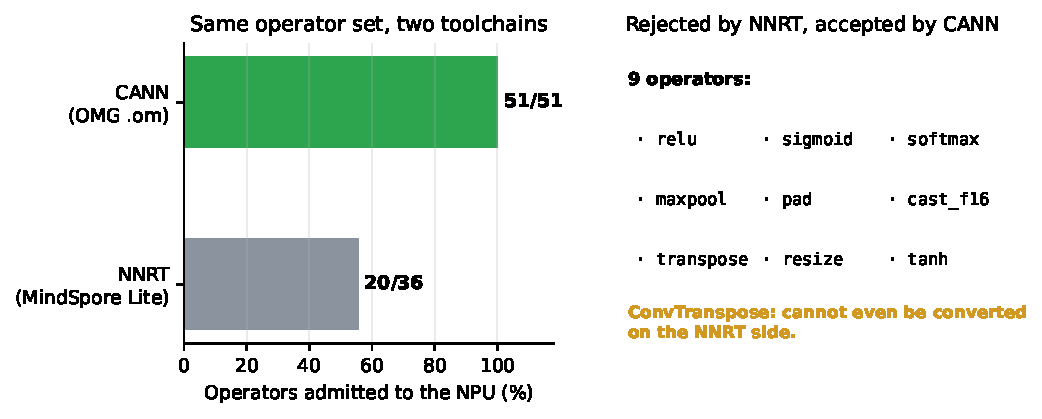
\includegraphics[width=\columnwidth]{fig2-operator-coverage.pdf}
\caption{The same operator family under two toolchains targeting the same
silicon. Left: fraction of operator probes admitted to the NPU. Right: the
operators rejected by NNRT in isolation but accepted by CANN.}
\label{fig:operators}
\end{figure}

A natural way to describe an NPU is by the set of operators it supports. We
argue this description is misleading, and that the useful object is the pair
(model, toolchain).

On the NNRT path, a set of 36 single-operator probes was compiled standalone and
classified by three signals (compilation success, graph build, and execution).
Twenty were accepted; sixteen were rejected, including operators as ordinary as
\texttt{ReLU}, \texttt{Sigmoid}, \texttt{Softmax}, \texttt{MaxPool},
\texttt{Pad}, \texttt{Cast}, \texttt{Transpose} and \texttt{Resize}. Taken at
face value, this says the accelerator cannot execute a rectifier.

It can. We compiled a larger set of 51 operator probes to CANN offline graphs
and ran each on the device through three gates (format compatibility, graph
construction and build, execution). All 51 passed every gate, including all nine
of the operators that the NNRT path rejects. One case is sharper still:
\texttt{ConvTranspose} cannot be \emph{converted at all} on the NNRT side---the
converter fails shape inference---yet converts and executes on the CANN side.
The same ONNX file fails to produce a model on one path and runs on the other.

\subsection{Mechanism, and its epistemic status}

The observations above are consistent with a specific mechanism. Operators that
are rejected in isolation are still carried onto the NPU when they appear as
fusion neighbours of an adjacent convolution. The supporting evidence is
indirect: residual and MobileNet-family networks contain many rejected operators
yet accelerate as a whole by $8$--$13\times$, and partition logs for such models
report subgraphs of the form \texttt{NPU:2, CPU:1} rather than the near-total
CPU partitioning that the standalone rejection rate would predict.

\textbf{We do not claim this mechanism has been causally established.} Doing so
requires a controlled experiment in which the weights are held fixed and only
the isolation of an operator is varied, and measuring the resulting partition
and latency. That experiment has not been run. The mechanism is offered as the
best current explanation of the correlation, and is flagged as such wherever it
is used.

\subsection{What this does and does not license}

The comparison licenses a statement about \emph{admission}: an operator's
absence from one toolchain's supported list is not evidence that the hardware
cannot execute it. It does not license a statement about \emph{speed}. On the
production configuration, MindSpore Lite was in fact faster than CANN for the
recognition model ($3.99$\,ms against $5.19$\,ms). The CANN-side latencies were
collected with three repetitions and no warm-up and are therefore used for
ordering only, never quoted as measurements.

\subsection{From probes to a production stage: gaining admission by re-architecting}

Operator probes establish \emph{where} the boundary lies. A more useful question
is what crossing it costs in practice. We answer it with one stage of the
pipeline studied in \S\ref{sec:pipeline}: vehicle detection, which dominates the
frame budget and is therefore the stage whose placement matters most.

The same task was implemented under two model architectures and compiled with
the same converter. The first, an ultralytics \texttt{v5-u} detector whose head
contains a distribution-focal-loss (DFL) projection, \emph{cannot be converted
at all}: shape inference fails on the DFL convolution
(\texttt{InferShapeByNNACL for op: /model.24/dfl/conv/Conv failed}) and the
converter aborts. This is not a tuning problem --- the DFL head's permutation is
part of the architecture.

The second architecture, the original anchor-based YOLOv5, is admissible but not
by default. Exported naively it fails the static gates: its detection head
performs \texttt{view}$\rightarrow$\texttt{permute}$(0,1,3,4,2)$ and carries
sigmoid and anchor-grid decoding on rank-5 tensors, whereas the compiler admits
only rank $\le 4$ and the permutation $[0,1,3,2]$. The failure is however
\emph{repairable}, because it lies in the decode stage rather than in the
architecture: cutting the graph at the last rank-4 tensor --- the head
convolution output --- and moving sigmoid and anchor decoding to the host leaves
a graph with no transposition and no tensor above rank 4. We verified the cut is
semantics-preserving by running both graphs under a common runtime and comparing
the decoded outputs element-wise (maximum relative deviation
$1.9\times10^{-5}$, i.e.\ float32 accumulation noise).

The re-architected detector converts cleanly, with no warnings, and lands on the
NPU: the observed backend string is
\texttt{NNRT:NPU\_ohos.boot.hardware.kirin8020\_v2\_0} with no fallback.
Bare-head latency is $5.39$\,ms against $42.02$\,ms for the same model on the
same stack's CPU, a ratio of $7.79\times$. Landing is self-evidenced twice over:
from the backend string, and from the fact that the NPU and CPU checksums
differ --- had the request silently fallen back, both would be bit-identical.

Two boundaries apply. First, these are \emph{bare-head} figures: they exclude
letterbox pre-processing, anchor decoding and non-maximum suppression, and must
not be divided into the in-pipeline figure of \S\ref{sec:pipeline}, which
contains work the accelerator does not perform. Second, the detector is not yet
integrated: its outputs are raw head tensors, and wiring it in is separate work.

The lesson generalises past this stage. An operator list describes the
\emph{hardware}; admission is decided by the (model, toolchain) pair; and where
the model is at fault, the fault may be architectural --- as with DFL, where no
rewriting of the graph helps --- or merely positional, as with a decode head,
which can be moved off the accelerator's critical path. Only the second is a
conversion problem.

% ============================================================================
\section{Case Study: A Four-Stage Licence-Plate Pipeline}
\label{sec:pipeline}

\begin{figure}[t]
\centering
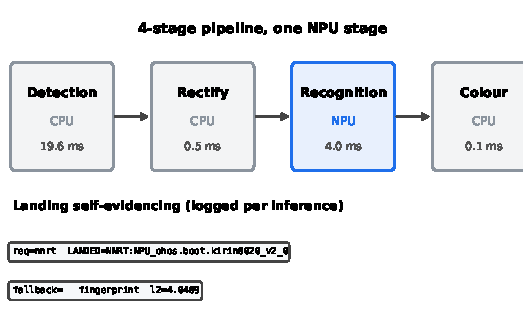
\includegraphics[width=\columnwidth]{fig1-pipeline-and-landing.pdf}
\caption{The four-stage pipeline and the per-inference landing record. Stage
timings are from the production configuration on a detected frame (median).}
\label{fig:pipeline}
\end{figure}

The application is a Chinese licence-plate recognition pipeline: detection,
perspective rectification, sequence recognition, and colour determination. The
colour stage is a pixel measurement rather than a classifier, after an
investigation established that a pre-trained colour classifier inherited from
earlier work was being decoded through a rotated label table---an error that had
been recorded as an unresolved disagreement between two components, and which
turned out to be an artefact of the decoding rather than a disagreement.

The pipeline is instrumented per stage, so that a single frame yields not one
end-to-end number but a budget: on a detected frame in the production
configuration, detection accounts for 49\% of the frame and recognition for
10\%. This decomposition is what makes the rest of the analysis actionable, and
it is also what refutes the framing the project began with: on this pipeline,
further NPU optimisation has a small ceiling, because the NPU-resident stage is
already the cheapest part of the frame.

\subsection{Does switching a backend change the answer?}

\begin{figure}[t]
\centering
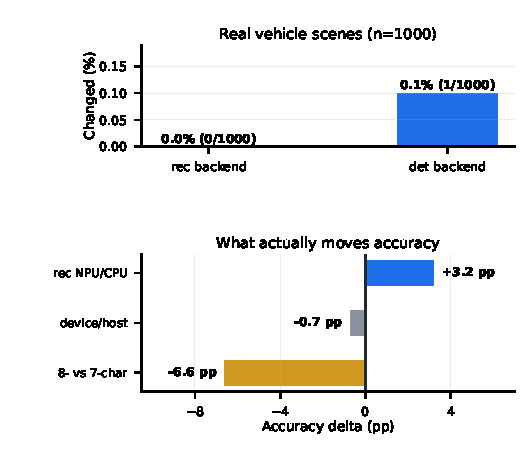
\includegraphics[width=\columnwidth]{fig3-backend-sensitivity.pdf}
\caption{Left: over 1{,}000 real vehicle scenes, switching a role's backend
almost never changes the output. Right: the quantities that do move accuracy,
including one that moves it in the opposite direction.}
\label{fig:sensitivity}
\end{figure}

We ran the same probe over the same 1{,}000 real vehicle images, changing the
backend of exactly one role at a time. Placement was confirmed different by the
landing record in each run. Over these images, switching the recogniser's
backend changed \emph{zero} outputs, and switching the detector's changed one
(0.1\%). The single disagreement was a case where both backends were wrong, and
wrong differently.

This is the result one wants, and it is also the result that is easiest to
over-read. Two further measurements prevent that.

\subsection{Low divergence does not imply absence of bias}

Accuracy on the same 1{,}000 images was $89.9\%$ for the NPU recogniser and
$86.7\%$ for the CPU recogniser. A difference of $3.2$\,pp would be unremarkable
if judged against independent confidence intervals, since the two measurements
share the images and therefore share the variance attributable to image
difficulty. A \emph{paired} McNemar test, which conditions on the discordant
pairs, gives $38$ images correct only on the NPU against $6$ correct only on the
CPU, $p<0.0001$. Both sessions used the same C++ pre-processing routine and the
same model file, so this is a pure backend effect.

The same test applied to the device-versus-host comparison is instructive in the
opposite direction. The device NPU recogniser scored $89.9\%$ against $90.6\%$
for the host reference implementation---a $0.7$\,pp gap, which an earlier
analysis of ours had reported as evidence that the port was faithful. The paired
test gives $0$ images correct only on the device against $7$ correct only on the
host, $p=0.0156$. The pairing is strictly nested: host $\supset$ NPU $\supset$
CPU. A gap of seven images is small and, for engineering purposes, acceptable;
but it is systematic, and ``faithful'' was the wrong word for it.

The general point is that divergence rate and bias are different quantities. A
divergence rate of 0.1\% that is consistently signed will accumulate into a
statistically significant accuracy difference over a thousand images. Reporting
only the divergence rate would have hidden this.

\subsection{The dominant variable is plate length, not placement}

\begin{figure}[t]
\centering
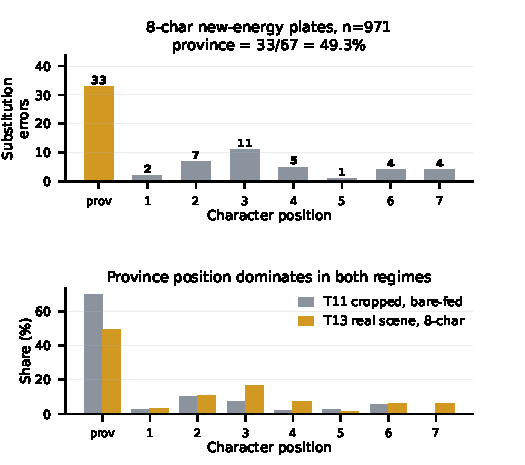
\includegraphics[width=\columnwidth]{fig4-error-position.pdf}
\caption{Substitution errors by character position. The province position
dominates across regimes, plate lengths and backends.}
\label{fig:errors}
\end{figure}

If backend placement is a second-order effect, what is first-order? Two
candidates were measured.

\textbf{Plate length.} On 1{,}000 eight-character new-energy plates from
CCPD-Green, the same pipeline scored $92.5\%$, against $99.1\%$ on
seven-character plates in the comparable real-scene run: a $6.6$\,pp cost for one
additional character, with the recogniser's backend divergence staying at 0.1\%.
Because the two datasets differ in province composition, a province-matched
control was run: all five provinces with sufficient samples moved in the same
direction, and the largest (Anhui, $n=600$) moved by $6.5$\,pp, essentially the
pooled figure. The cost is attributable to plate length.

\textbf{Dataset skew.} We had hypothesised that the province skew of the
inherited benchmark ($956/1000$ Anhui) was inflating the reported accuracy. On a
26-province balanced set ($n=3368$) the hypothesis was refuted: accuracy was
$90.9\%$ against $90.6\%$. What skew changes is not \emph{how much} is wrong but
\emph{where}: on the skewed set, 89\% of failures fell on the province position;
on the balanced set the province position accounted for a far smaller share and
errors moved into the middle of the string. This is a more useful finding than
the one we set out to test, and it is the reason the error-position analysis in
Fig.~\ref{fig:errors} is reported per regime.

Across four independent measurements---cropped images fed directly to the
recogniser, cropped images through the full pipeline, real vehicle scenes, and
eight-character plates---the province position remained the largest single error
site ($75/77$, $5$ of $9$, and $33/67 = 49.3\%$ respectively), while switching
backends left the error pattern essentially unchanged. The province position is
a property of the recogniser and the data, not of the accelerator.

% ============================================================================
\section{Sustained-Load Behaviour}
\label{sec:rq4}

\begin{figure}[t]
\centering
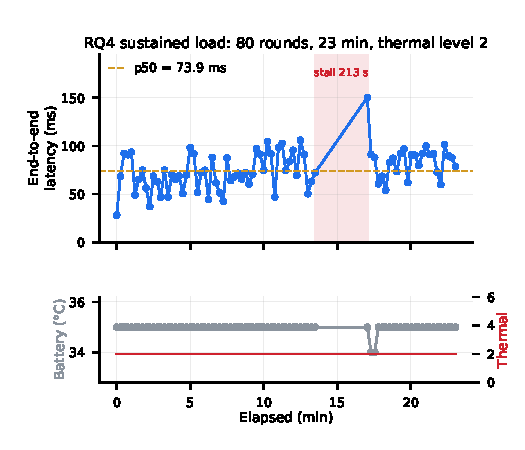
\includegraphics[width=\columnwidth]{fig5-rq4-sustained.pdf}
\caption{Sustained load over 80 rounds (23.3 min). Thermal level never leaves
level~2 and the tensor fingerprints are constant in every round, yet latency
drifts upward. The shaded region is a 213\,s stall in which the operating system
froze the application; it is marked rather than removed, because a reader who
did not know about it would read it as a latency spike.}
\label{fig:rq4}
\end{figure}

The fourth question is whether an accelerator's advantage survives sustained
load. On this platform that question is usually framed thermally: the system
exposes eight load levels, and the vendor requires that non-essential background
work stop from level three upward. A previous characterisation of the same
device family reported a $15$--$20\%$ NPU latency penalty when the thermal level
moves from 2 to 3, which makes the crossing a natural quantity to measure.

We ran the production pipeline for 80 rounds at 15\,s intervals, 23.3 minutes in
total, recording thermal level, battery temperature, state of charge, charging
state and the landing fingerprints on every round.

\subsection{The thermal regime was not reached}

The thermal level was \emph{constant at 2 for all 80 rounds}; battery
temperature stayed within 1\,$^\circ$C. The 2$\to$3 crossing was never reached,
so the $15$--$20\%$ penalty rule is neither confirmed nor refuted here. An
earlier 25-round run of the same probe had the same outcome at thermal level~1
over 6 minutes; extending the run by a factor of four did not change it. We
report this as a negative result rather than extrapolating.

\subsection{Latency degrades without a thermal crossing}

The reason the negative result matters is that latency nevertheless drifted
upward, monotonically, over the run:

\begin{table}[t]
\caption{Latency drift across the sustained run, excluding the frozen interval.
Thermal level 2 and battery temperature 35\,$^\circ$C throughout.}
\label{tab:drift}
\centering
\begin{tabular}{lccc}
\toprule
& rounds 0--17 & rounds 36--53 & change \\
\midrule
End to end (mean) & 64.44 ms & 81.76 ms & $+26.9\%$ \\
CPU-resident stages & 49.47 ms & 63.94 ms & $+29.3\%$ \\
NPU-resident stage & 14.92 ms & 17.78 ms & $+19.2\%$ \\
\bottomrule
\end{tabular}
\end{table}

Two things follow. First, \textbf{a stable thermal level does not imply stable
performance}; a measurement protocol that records only thermal state and assumes
the rest is stationary will be wrong by roughly a quarter over twenty minutes.
Second, the degradation is \emph{not} uniform across the pipeline: the
CPU-resident stages degrade by $29.3\%$ against $19.2\%$ for the NPU-resident
stage. Since the production configuration places detection on the CPU, this is
consistent with the frame-budget analysis in \S\ref{sec:pipeline} and reinforces
the same conclusion from a different direction: on this pipeline, the
accelerator is not where the variability lives.

We do not attribute the drift to a mechanism. The device does not expose clock
or thermal-zone readings to applications, so frequency scaling, scheduler
behaviour and background interference cannot be separated here.

\subsection{Two protocol defects found while running this}

\textbf{The operating system freezes long-running foreground applications.}
Between rounds 54 and 55 the interval was 213\,s rather than 15\,s. The device
log shows the application being re-activated by the window manager at the end of
that interval, implying it had been backgrounded and frozen. This is the same
failure mode we had previously observed with screenshot capture. The remedy is
to override the screen-off timeout before starting the run
(\texttt{power-shell timeout -o}, restored afterwards); a rule of ``do not take
screenshots'' is insufficient, because the trigger here was the screen turning
off, not a screenshot. We mark the interval in Fig.~\ref{fig:rq4} rather than
removing it, and we exclude it from Table~\ref{tab:drift}.

\textbf{Inter-run variance is not a stable quantity at this sample size.} We
initially intended to report whether the NPU-resident or CPU-resident stages
exhibit more round-to-round variance, following the observation in prior work
that CPU-side variance is the larger. Across three measurements of the same
quantity we obtained three different answers: CPU-dominant, approximately equal,
and NPU-dominant. Segment-wise, the NPU-side coefficient of variation ranges
from $8.8\%$ to $48.2\%$ within a single run. We therefore report no comparison
of this kind. Answering it requires repeated measurements \emph{within} a round
rather than one measurement \emph{per} round, which the probe's design does not
provide. What can be stated is simply that round-to-round variance is large
(coefficient of variation around $27\%$), which is why single-point latency
figures are not usable as results on this platform.

% ============================================================================
\section{Discussion and Threats to Validity}
\label{sec:discussion}

\begin{figure}[t]
\centering
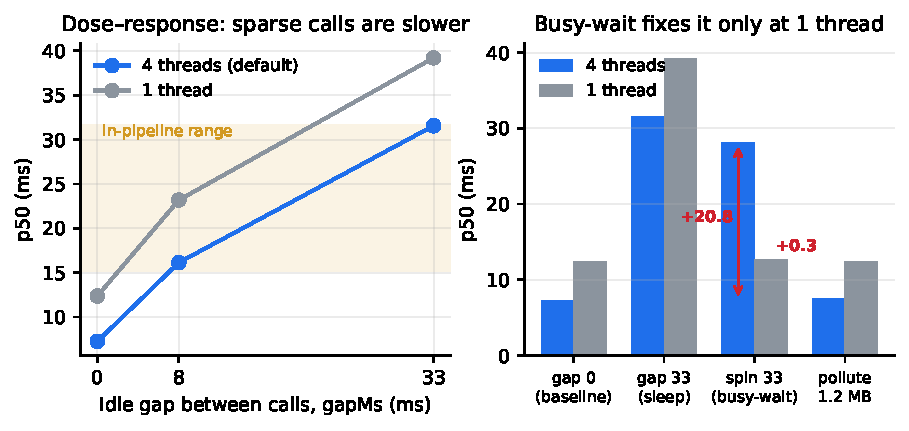
\includegraphics[width=\columnwidth]{fig6-c8-dose-response.pdf}
\caption{Why an isolated benchmark is not the product-path cost. Left: raising
the idle gap between calls from $0$ to $33$\,ms raises the median from
$7.26$\,ms to $31.56$\,ms, and the upper end of that range coincides with the
in-pipeline measurements. Right: a busy-wait of the same duration does not
recover the loss at four threads ($+20.8$\,ms) but almost fully recovers it at
one ($+0.29$\,ms), separating frequency scaling from thread-pool wake-up.}
\label{fig:c8}
\end{figure}

\textbf{Isolated benchmarks are not product-path costs.} A discrepancy we did
not expect, and which changed how we read every other latency number, is that
the same model on the same backend with the same thread count costs roughly
twice as much inside the application as in an isolated probe: $19.5$--$31.6$\,ms
in the pipeline against $7.4$\,ms in a tight loop (Fig.~\ref{fig:c8}). A three-step experiment
isolated two additive mechanisms. A dose--response sweep showed that increasing
the idle gap between calls raises the median from $7.26$\,ms (no gap) to
$16.14$\,ms ($8$\,ms) to $31.56$\,ms ($33$\,ms)---and the $33$\,ms point lands
inside the observed in-pipeline range. Replacing the sleep with a busy-wait of
the same duration did \emph{not} restore performance at four threads, which
rules out frequency scaling as the sole cause. Repeating at one thread, where
there is no worker pool to park, restored it almost completely (a residual of
$+0.29$\,ms against $+20.8$\,ms at four threads). The two mechanisms are
therefore frequency scaling, which is not controllable from the application, and
thread-pool wake-up latency, which is controllable only by keeping threads busy
---a remedy that would violate the platform's rule against sustained background
computation. The practical consequence is that an isolated microbenchmark must
not be quoted as the cost of a stage in a deployed pipeline.

\textbf{Throughput claims require knowing what limits the measurement.} In the
camera path, arrival rate and completion rate are equal and no frames are
dropped, which is naturally read as ``the pipeline keeps up with the camera''.
It is not a valid inference: when the pipeline is the slower party, the receiver
buffer fills and the camera stops delivering, so the discarded frames are never
counted as dropped. The distinction requires a control configuration that
acquires frames without inference; under that control the camera supplied
$49.98$\,fps, while the same configuration with inference reached $36.2$\,fps
(production) and $43.6$\,fps (all-NPU). The pipeline was the limit, and the
arrival rate was reporting our own consumption.

\textbf{Cross-stack comparability.} As stated in \S\ref{sec:protocol}, only
same-stack ratios are comparable. We report a $4.46\times$ speed-up for the
recogniser (same stack, same pre-processing, same model file, $16.78$\,ms
against $3.76$\,ms); we do not report cross-stack speed-ups as results.

\textbf{What the fingerprint does not prove.} The tensor fingerprint establishes
that a backend executed. It does not establish that the computation was correct.
Correctness is established only against human-annotated ground truth. We note
this because our own project contains a case where the fingerprint was initially
read as evidence about the accelerator when it was in fact evidence about our
own input tensor: a padding region in a pre-processing routine was not being
zeroed, so a preceding run through a differently-laid-out buffer left residue in
it. The output-layer symptom was a plausible-looking plate string missing one
character. The fingerprint faithfully recorded that something changed; only
aligning the session timeline showed that the something was on our side.

\textbf{Scale and generality.} All results are from one device, one OS version,
and one application. The 1{,}000-image sets are single-source, and the
eight-character set is 60\% Anhui, a skew that cannot be removed by sampling
because the source data is itself skewed. The cross-SKU question---whether these
findings hold across the 9010/9020/9030 parts---was deliberately scoped out
because it depends on retail demonstration devices whose availability, thermal
state and charging state we cannot control.

% ============================================================================
\section{Conclusion and Future Work}

We set out to answer a question that this platform makes surprisingly hard: did
the accelerator actually execute the work? The answer we can support is that
placement can be established from raw logs, provided the request, the outcome
and any fallback are recorded separately and corroborated by a differential
against the CPU. Doing so caught a real defect, and---at least as usefully---it
caught us over-claiming what the fingerprint proves.

Applying the protocol produced a result that is more useful than a speed-up
table. For this pipeline, backend placement is nearly inert: it changes almost
no outputs, and where it does bias accuracy, it does so by a few percentage
points. Plate type and plate length move accuracy by considerably more. The
engineering conclusion is that effort spent re-validating outputs after a
backend switch is largely misdirected, whereas effort spent on coverage---which
plate types, which provinces---is not.

Three directions remain open, and we prefer to name them than to imply they are
done. The fusion-carry-over mechanism requires a controlled experiment with
fixed weights and varied operator isolation before it can be stated as causal.
The sustained-load question---whether the NPU's advantage survives a thermal
soak---requires a longer run than the one we report, and is not answered here.
And the cross-SKU scaling question requires hardware we cannot control.

% ============================================================================
\begin{thebibliography}{1}

\bibitem{laskaridis2024melt}
S.~Laskaridis, K.~Katevas, L.~Minto, and H.~Haddadi, ``MELTing Point: Mobile
Evaluation of Language Transformers,'' in \emph{Proc. 30th Annu. Int. Conf.
Mobile Computing and Networking (MobiCom '24)}, 2024, pp. 890--907.
doi: 10.1145/3636534.3690668.

\bibitem{xu2018ccpd}
Z.~Xu, W.~Yang, A.~Meng, N.~Lu, and H.~Huang, ``Towards End-to-End License
Plate Detection and Recognition: A Large Dataset and Baseline,'' in
\emph{Proc. European Conf. Computer Vision (ECCV)}, 2018, pp. 255--271.

\bibitem{zherzdev2018lprnet}
S.~Zherzdev and A.~Gruzdev, ``LPRNet: License Plate Recognition via Deep Neural
Networks,'' arXiv:1806.10447, 2018.

\bibitem{silva2018unconstrained}
S.~M.~Silva and C.~R.~Jung, ``License Plate Detection and Recognition in
Unconstrained Scenarios,'' in \emph{Proc. European Conf. Computer Vision
(ECCV)}, 2018, pp. 580--596. doi: 10.1007/978-3-030-01258-8\_36.

\bibitem{laroca2018robust}
R.~Laroca, E.~Severo, L.~A.~Zanlorensi, L.~S.~Oliveira, G.~R.~Gon\c{c}alves,
W.~R.~Schwartz, and D.~Menotti, ``A Robust Real-Time Automatic License Plate
Recognition Based on the YOLO Detector,'' in \emph{Proc. Int. Joint Conf. Neural
Networks (IJCNN)}, 2018.

\end{thebibliography}

\end{document}
